\documentclass[fleqn]{jbook}
\usepackage{physpub}

\begin{document}

\begin{question}{専攻 問題6}{}

\def\CuK{${\rm Cu-K}_{\alpha}$}
\def\MoK{${\rm Mo-K}_{\alpha}$}

X線の吸収に関する実験について次の問いに答えよ。

\begin{subquestions}
\SubQuestion
  単色化した \CuK 線(波長$\lambda_{K}=0.1542\Unit{nm}$) を
  コリメーターを用いて細いビームにし、その強度を充分広い検出窓を持つ
  シンチレーションカウンターで測定する図1のような装置を作った。
%
  \begin{center}
    \fbox{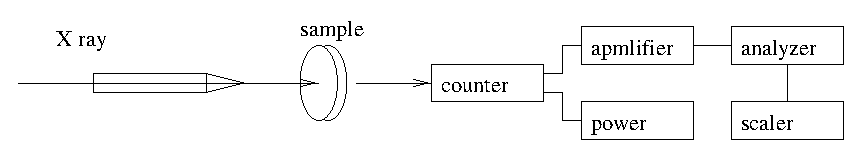
\includegraphics[clip]{1994phy6-1.eps}}
  \end{center}
%
  \parbox[t]{98mm}{
  このビームの中に表面積の充分大きい、$0.1\Unit{mm}$の一様な厚さを
  持つシリコン薄板試料をその表面がビームに垂直になるようにセットして、
  その枚数$n$を変えながら透過するビームの強度$I$を測定し右の表の結果
  を得た。また、シリコンのかわりにX線を通さない鉛板を置いてバック
  グラウンドを測定した結果、$60$秒間に$98$カウントが計測された。
  入射強度$I_{0}$のX線が、吸収係数$\mu$、厚さ$t$の物質を透過した後の
  強度は $I = I_{0} \exp{(-\mu t)} $ と表される。実験結果に関する
  次の問に答えよ。ただし、
  $\ln{10}=2.30$、$\log_{10}{2}=0.301$、$\log_{10}{3}=0.477$とする。
%
  }\parbox[t]{62mm}{\vspace*{-5mm}
%
  \begin{center}
  \begin{tabular}{|crc|}\hline 
  $n$(枚)& $I$(カウント) & 測定時間(秒) \\
     0   &  78,018 &   1   \\
     1   &  48,106 &   1   \\
     2   &  18,065 &   1   \\
     3   &  22,195 &   5   \\
     4   &  10,891 &  10   \\
     5   &   8,010 &  30   \\
     6   &   3,924 &  60   \\ \hline
  \end{tabular}
  \end{center}
  }

  \begin{subsubquestions}
  \SubSubQuestion
    実測した透過ビーム強度をシリコン薄板の厚さ$t$に対して調べてみると、
    枚数が少ないとき実測値は上の式からはずれている。その原因は何か
    議論せよ。

  \SubSubQuestion
    シリコンの吸収係数$\mu \Unit{[mm^{-1}]}$、および入射強度$I_{0}$
    [カウント/秒] を、$10\%$程度の精度で求めよ。

  \SubSubQuestion
    厚さ$0.025\Unit{mm}$の金属薄膜を{\bf 1}と同じ条件のX線ビームの
    中に挿入してその透過強度を測定したところ、10秒間に30,300
    カウント計測された。この金属の吸収係数を求めよ。また、次の各金属
    の \CuK 線に対する吸収係数 $\Unit{(mm^{-1})}$ の値を参照
    して、この金属は次のうちどれか推定せよ。
%
    \begin{center}
    \begin{tabular}{llllll}%
      Ti (93) &  V (136) & Cr (186) & Fe (255) &  Co (315) & Ni (44) \\
    \end{tabular}%
    \end{center}
  \end{subsubquestions}

\SubQuestion
  使用するX線を \CuK 線から \MoK 線(波長$0.0711\Unit{nm}$) に換えた
  とき、正しく信号を取り出すためにシンチレーションカウンターの計測
  回路中調整すべき点を挙げよ。

\SubQuestion
  \parbox[t]{103mm}{
  試料として銅の薄膜を用い、今度は入射X線の波長を連続的に変化させ
  ながらその透過強度を測定し右図の結果を得た。

  \begin{subsubquestions}
  \SubSubQuestion
    図中で波長$\lambda_{a}=0.1381\Unit{nm}$に見られる大きな強度の
    不連続点は何と呼ばれるか。

  \SubSubQuestion
    {\bf 1}におけるX線発生管の銅のターゲットから発生する\CuK 線
    (波長$\lambda_{K}=0.1542\Unit{nm}$) とこの
    $\lambda_{a}=0.1381\Unit{nm}$
    との間には$\lambda_{K}>\lambda_{a}$の関係があるが、このことをX線
    の発生を吸収の機構をもとに説明せよ。

  \end{subsubquestions}

  }\parbox[t]{58mm}{
  \begin{center}
    \mbox{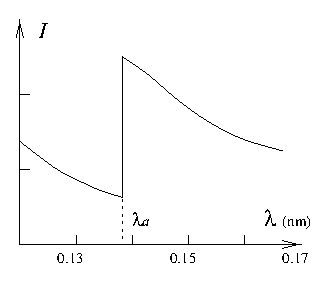
\includegraphics[clip]{1994phy6-2.eps}}
  \end{center}}

\end{subquestions}
\end{question}
\begin{answer}{専攻 問題6}{}
\def\CuK{${\rm Cu-K}_{\alpha}$}
\def\MoK{${\rm Mo-K}_{\alpha}$}

\begin{subanswers}
\SubAnswer
  \begin{subsubanswers}
  \SubSubAnswer
    シンチレーションカウンターには不感時間があり、一つのパルスを
    発生してから次のパルスを発生させるまでにおよそ$2\Unit{\mu s}$
    ほどかかる。この間に入ったパルスは無視されるので、枚数が少なく
    計数が多い時には数え落しが多くなる。

  \SubSubAnswer
    横軸にシリコンの厚さ$t\Unit{[mm]}$ 、縦軸に入射強度
    $I$[カウント/秒] をとると以下のようになる。
%
    \begin{center}
      \mbox{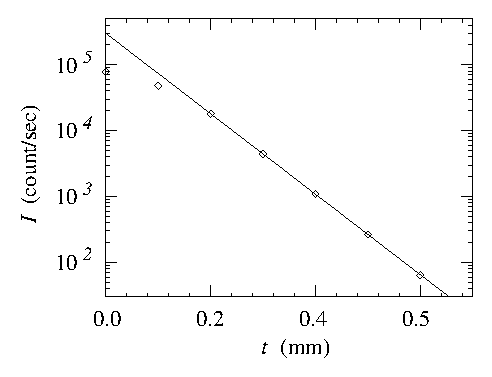
\includegraphics[clip]{1994phy6-3.eps}}
    \end{center}
%
    この傾きおよび切片から、$\mu = 14\Unit{[mm^{-1}]}$、
    $I_{0}= 3.0\Keta{5}[カウント/秒]$ と求められる。

  \SubSubAnswer
    求める吸収係数を$\mu_{0}\Unit{[mm^{-1}]}$ とすると、{\bf 1} と
    同じ条件であることから、
%
    \[ I_o \exp{(-0.025 \mu_{0})} = \frac{30300}{10}-\frac{98}{60}%
       \hspace{15mm}% 
       \mu_{0} = 1.8\Keta{2} \]
%
    したがって、この金属はCrと推定される。

  \end{subsubanswers}

\SubAnswer
  \MoK 線の方が \CuK 線よりも波長が短いので、フォトンのエネルギーは
  高く、電圧の高いパルスとして観測される。したがって、シグナルとノイズ
  を選別するためのパルス波高の閾値を高くしておかなければならない。

\SubAnswer
  \begin{subsubanswers}
  \SubSubAnswer
    吸収端(absorption edge) 

  \SubSubAnswer
    $\lambda<\lambda_{a}$の時には光電効果でK殻の電子をたたき出せるよう
    になるので急激に透過強度は減少する。したがって、K殻のエネルギーを
    $-E_{K}$とすると、
%
    \[ \lambda_{a} = \frac{hc}{E_{K}} \]
%
    また、特性X線 ${\rm K}_{\alpha}$ 線はK殻にできたホールにL殻から
    電子が落ち込む時に発生するので、L 殻のエネルギーを$-E_{L}$と
    すると、
%
    \[ \lambda_{K} = \frac{hc}{E_{K}-E_{L}} \]
%
    したがって、$\lambda_{K}>\lambda_{a}$である。

  \end{subsubanswers}
\end{subanswers}
\end{answer}


\end{document}
